\documentclass[varwidth]{standalone}

\providecommand{\packageName}[1]{PowerEdu.jl}
\providecommand{\packageNameNoJL}[1]{PowerEdu}
\providecommand{\powerflow}[1]{Power Flow}
\providecommand{\sparse}[1]{Sparse Power Flow}
\providecommand{\cpf}[1]{Continuation Power Flow}
\providecommand{\se}[1]{State Estimation}
\providecommand{\opf}[1]{Optimal Power Flow}

\usepackage{lipsum}
\usepackage{dirtree}
\usepackage{graphicx}
\usepackage{svg}

\providecommand{\figdir}{../../figures}
\providecommand{\imagedir}{../../images}

\begin{document}

\section{User Interface}

Upon downloading \packageName{} on their machine, the user will interact with the following directory heirarchy. For the sake of clarity, folders pertaining only to the IEEE\_14 Bus test case are shown, however, in general, every test case will have its dedicated folders for inputs and outputs.

\subsection{Directory Structure}

\dirtree{%
.1 {root (\packageNameNoJL{})}.
.2 {data}.
.3 {IEEE\_14}.
.4 {IEEE\_14\_Data.txt}.
% .3 {$\ldots$ (remaining test cases)}.
.2 {processedData}.
.3 {IEEE\_14}.
.4 {BusDataCard\_pu.csv}.
.4 {BranchDataCard\_pu.csv}.
.4 {YBus.csv}.
.4 {$\ldots$ (other generated files)}.
% .3 {$\ldots$ (remaining test cases)}.
.2 {src}.
.3 {ContinuationPowerFlow.jl}.
% .3 {HelperFunctions.jl}.
.3 {IEEE\_CDF\_Parser.jl}.
% .3 {JacobianBuilder.jl}.
% .3 {LU\_Factorization.jl}.
.3 {OptimalPowerFlow.jl}.
.3 {PowerFlow.jl}.
.3 {SparsePowerFlow.jl}.
.3 {StateEstimation.jl}.
.3 {$\ldots$ (other modules)}.
% .3 {YBusBuilder.jl}.
.2 {main.jl}.
.2 {main\_notebook.jl}.
.2 {README.md}.
.2 {LICENSE}.
}

\subsection{Pluto Interactive Notebook}

While users are free to make function calls from \packageName{} within any editor of their choice, we also provide a handy interactive notebook environment for users to quickly get an overiew of the package using already made scripts with easy to manipulate control widgets. We prefer Pluto.jl \cite{PlutodotjlGithub} as the notebook environment instead of other popular notebook environments like Jupyter or Observable because, unlike Observable, it is an open source notebook environment and and more importantly, unlike Jupyter it is a reactive notebook, i.e. it does not have any hidden states in the workspace \cite{Pimentel2019May, Perkel2021May}.


\includegraphics[width=0.4\textwidth]{\imagedir/plutoImg01}
% 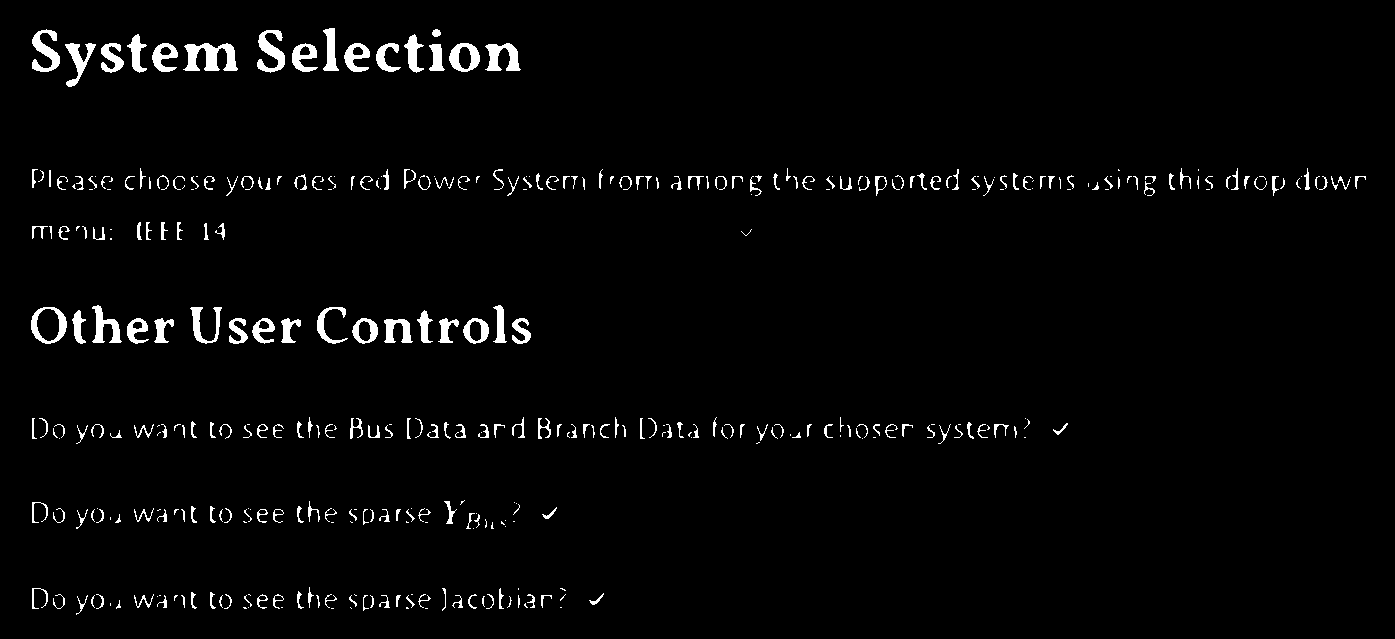
\includegraphics[width=0.5\textwidth]{\figdir/plutoImg03}
% \includesvg{\figdir/plutoImg02}

\ifstandalone
\bibliographystyle{IEEEtran}
\bibliography{../../outputs/BiBFile}
\fi

\end{document}